\chapter{Background and Related Work}

This chapter begins by describing what social networks are and what features one can expect to find in them. In particular, the features of two of the largest social networks, Facebook and Twitter, are discussed in detail, including how those features might be useful in recommending novel content to users. Using this description for background, the discussion then moves to research that has already been done in this field and which techniques for content recommendation have shown promise so far.

\section{Social Networks}

Facebook and Twitter are certainly the most popular social networking services, with more than 1 billion user accounts between them. There are dozens of other social networks, however, including many with millions of users such as Google+, Pinterest, and LinkedIn. It would be impractical and of limited value to discuss the nuances of all of these services and to what degree they implement particular features, but some background is necessary in order to understand the work undertaken in this project. Because Twitter and Facebook are the most popular social networking services and demonstrate all of the common features of social networks this discussion will be limited to only these two services.

Before describing these two services and their features in detail, it is valuable to begin with a brief discussion of the general features that are common to all social networks. Examining these general features provides a good basis for comparison of how the general features are implemented by the two test cases. It is also helpful as a reference to show that while the study undertaken for this project was specific to one particular social networking service, the features used were actually quite generic and could easily be extended to other services.


\subsection{What are Social Networks?}

At its core, a social network is a set of users, a set of edges connecting those users, and content produced by those users. Depending on the network and the relationships between users, the edges may be either directed or non-directed, and sometimes a given network may include edges of both types. A non-directed edge indicates that both users are subscribed to each other's content while a directed edge from user A to user B indicates that while user A is subscribed to content produced by user B and will see all public content from user B, user B will not see any content from user A.

The types of content produced also vary depending on the network. Twitter famously limits content to 140 characters of text, a limit designed to ensure that it can fit within the standard text message size limit of 160 characters. Still, those 140 characters can contain links to any other sort of content, and as the service has developed various conventions have been created in an ad hoc manner by its users in order to mark up the text to provide additional meaning. Facebook users, meanwhile, can share much longer text updates, photos, links, and videos. 

Another common feature of social networks is the ability for users to create profiles to tell other users about themselves and to express their interests and desires. The importance of that profile depends on the network, and in some cases it is the primary form of content produced by users. LinkedIn, for example, is a social network designed for professional networking and job-seekers, and its user profile pages are essentially just extended CVs.

Social networks also frequently provide the ability for users to re-share or forward content from other users so that their connections can see that content. This allows links and pictures to make their way across the network and be seen by users who are not themselves connected to the original user who produced a piece of content. And, importantly for the task of recommending content, it provides a good insight into the types of content that the person re-sharing the content finds interesting.

The degree to which networks support these features varies widely, but most networks---and certainly the majority of the most popular networks---implement all of these features.

\subsection{Facebook}

Facebook was originally founded as a way for students at Harvard University to keep in contact with each other. Early versions of the website were rudimentary compared to the current behemoth---the only real features were the ability to become friends with other users and to fill out a profile indicating the user's birth date, home town, current location, interests, and similar biographical details. From those early beginnings the network expanded first to other universities and then to secondary schools before membership was eventually open to everyone.

As one of the oldest social networks which still enjoys a large user-base, Facebook has evolved quite a bit over the years since it was created. As other social networks have challenged it by introducing new features, Facebook has responded by adding versions of those same features with slight modifications to adapt them to the Facebook environment. Over the years of growth the modern version of Facebook has  slowly taken shape as features such as photo sharing, the news feed, and the `like button' have been introduced.

\subsubsection{Features}

The Facebook network is built around the concept of friends. The edges in the Facebook network are connections between users who (mostly) know each other in real life and are bi-directional. One user sends a friend request to a second user and if the second user accepts then the connection is created and each user can see content produced by the other.

Suppose that there is a user Alice who is friends with a user named Bob but not with a user named Carol. Bob, however is friends with Carol. Alice might share a piece of content $C_{A}$ with her friends, in which case Bob will see the update but Carol will not. Similarly, if Carol shares a piece of content $C_{C}$, Bob will see it but Alice will not. Finally, if Bob shares a piece of content $C_{B}$, both Alice and Carol will see it since both users are friends with Bob. This visibility is shown in Figure~\ref{fig:fb_content_visibility}.

\begin{figure}
  \centering
\begin{displaymath}
  \xymatrix{
    Alice \ar@<0.5ex>[r] & C_{A} \ar@{.>}@<0.5ex>[l] \ar@{.>}[dl] \\
    Bob \ar@{<-->}[u] \ar@{<-->}[d] \ar@<0.5ex>[r] & C_{B} \ar@{.>}@<0.5ex>[l] \ar@{.>}[ul] \ar@{.>}[dl]\\
    Carol \ar@<0.5ex>[r] & C_{C} \ar@{.>}@<0.5ex>[l] \ar@{.>}[lu] }
\end{displaymath} 
  \caption[Visibility of content on Facebook]{An example of how visibility of content works on Facebook. The dashed edges indicate the friendship connections between users. Directed edges from users to content indicate authorship, and dotted directed edges from content to users indicate which users can see that content.}
\label{fig:fb_content_visibility}
\end{figure}

The primary forms of content on Facebook are status updates, photographs, and links. Status updates are just text updates, sometimes telling other users what that person is doing, sometimes asking for advice, and sometimes just expressing emotions. Photographs and links are both self-explanatory, and are usually accompanied by captions or explanatory text from the user describing his or her thoughts on the content being shared. Each of these types of content is accompanied by a set of comments made by friends. Additionally, friends may 'like' the content by pressing the `like' button to indicate some sort of agreement, support, or genuine like of the associated status, link, or photograph without needing to leave a comment.

More recently, perhaps in response to competition from Twitter, Facebook has introduced the ability to share (forward) content from another user and to subscribe to public posts of another user or group, essentially creating a directed edge between those users. Returning to the example of Alice, Bob, and Carol, if Alice shares content $C_{A}$, Bob will see it but Carol will not since Alice and Bob are friends while Alice and Carol are not. Bob can re-share this, however (provided that Alice's privacy settings allow this) at which point Carol will be able to see it. This visibility relationship is shown in Figure~\ref{fig:fb_reshare}. Additionally suppose that Carol subscribes to the public updates of Alice. In this case, if Alice shares a photograph publicly, Carol will be able to see it without Bob having to re-share it since she subscribes to Alice's public updates. 

\begin{figure}
  \centering
  \begin{subfigure}[b]{0.3\textwidth}
    \centering
    \begin{displaymath}
    \xymatrix{
    Alice \ar@<0.5ex>[dr] &  \\
    Bob \ar@{<-->}[u] \ar@{<-->}[d]  & C_{A} \ar@{.>}@<0.5ex>[ul] \ar@{.>}[l] \\
    Carol  & }
    \end{displaymath}
    \caption{Before Bob reshares $C_{A}$}
    \label{fig:fb_reshare_before}

  \end{subfigure}
  \quad
  \begin{subfigure}[b]{0.3\textwidth}
    \centering
    \begin{displaymath}
    \xymatrix{
    Alice \ar@<0.5ex>[dr] &  \\
    Bob \ar@{<-->}[u] \ar@{<-->}[d] \ar@<0.5ex>[r] & C_{A} \ar@{.>}@<0.5ex>[ul] \ar@<0.5ex>@{.>}[l] \ar@{.>}[dl] \\
    Carol  & }
    \end{displaymath}
    \caption{After Bob reshares $C_{A}$}
    \label{fig:fb_reshare_after} 
  \end{subfigure}
  \caption[Visibility of reshared content on Facebook]{Visibility of content on Facebook before and after content is reshared. The dashed edges indicate the friendship connections between users. Solid edges between users and content indicate content authorship and resharing, and dotted edges between content and users indicate visibility. This figure does not include the situation where Alice subscribes to the public updates of Carol. }
  \label{fig:fb_reshare}
\end{figure}


As alluded to above, various privacy controls have been put in place over the years to give users control over who can see what content. Though the original idea of Facebook was that friends on Facebook would correspond to friends in real life, the actual mode of use didn't follow and people often found themselves in nominal `friendships' with acquaintances or people from different social circles with whom they didn't necessarily want to share all of their content. Thus, users can choose to share specific content only with specific sets of people and to restrict the re-sharing of their content. Additionally, users must decide whether posts will be public, visible only to friends, or visible only to specific friends.

Other popular features of Facebook allow users to create events and send invitations to their Facebook friends and the ability to run applications and games developed by third-party developers which leverage the user's social data to provide additional experiences.

\subsubsection{Content Recommendation}
\label{sec:FbContentRec}

Many of the basic features of Facebook would be very applicable for use in a content recommendation scheme. The basic edges between users present an obvious starting point, but other features could be leveraged to put a more accurate weight on edges between users. Users who frequently comment on one another's posts are more closely connected than users who never interact, for example.

Similarly, if a user likes a post or comments on it then it indicates that the content itself was relevant to that user, information which could be used to recommend future content of interest to that user. Attending common events would be another method of determining just how close two nominal 'friends' actually are---users who go to the same events in the real world are obviously much more likely to be good friends than users who do not.

The large amount of information on a Facebook user's profile is another piece of information that could be leveraged to recommend content. If two users declare similar interests on their user profile then it would be more likely that those users would be interested in content generated by one another.

Facebook itself has developed a system based on many of these components to help it recommend other users that it believes you may know and want to become friends with. One such project is described in \cite{Backstrom2011}.

The major drawback to studying content recommendation on Facebook is that the data is difficult to access. Most of the content created by users and the edges between those users are private and thus inaccessible to researchers. Therefore most studies focusing on Facebook, including that in \cite{Backstrom2011}, are undertaken at least in part by employees of Facebook participating in research and development to help advance the interests of the company.

The private nature of this data made it unsuitable for study in this dissertation, though many of the other components of the network would have provided a rich set of features to use in content recommendation. Facebook is discussed here to show that it has analogues to most of the major features of Twitter and that all of the research undertaken in this dissertation could easily be applied to Facebook if the data were available.

\subsection{Twitter}

\subsubsection{History}

Created in 2006, Twitter is a social network noted for the brevity of its content. The basic concept is simple: users provide updates on what they are doing or thinking in up to 140 characters. The basic interface has changed very little since its inception and the feature set is still very similar to its beginnings, in marked contrast to the large number of features that are integrated into Facebook.

The original intent was that users could update their status and receive statuses from friends using SMS messages from their mobile phones, and thus the length of any given Twitter message was limited to be smaller than the maximum size of an SMS message, 160 characters.

The nature of the network began to change as smartphones---mobile phones capable of running applications and communicating with the internet---became ubiquitous following the release of Apple's first iPhone in 2007. Twitter provides an extensive Application Programming Interface (API), which has allowed application developers to create rich and visually pleasing interfaces to the service that have helped boost its popularity by making it even easier to use. As smartphones grew in popularity the need for and popularity of status updates via SMS faded, though the 140 character limit has remained.

Today, Twitter has over 140 million active users worldwide, and those users produce hundreds of millions of status updates each day. As a result, numerous attempts have been made to make sense of this vast source of public data about the feelings and activities of millions of people around the world. Research into this area is discussed in greater depth in Section~\ref{sec:InfoGatheringResearch}.

\subsubsection{Features}

Twitter updates are commonly known as \emph{tweets}, and the act of producing one is known as \emph{tweeting}. Within the research literature on Twitter, one person's \emph{Twitter feed}, the collection of all of the tweets that they have produced, is commonly called a microblog in reference to the previously mentioned 140 character limit imposed on each tweet. Edges between users are directed. If a user Alice follows a user named Bob but Bob does not follow Alice, Alice will see all of Bob's tweets, but Bob won't see any of Alice's tweets. This is shown in Figure~\ref{fig:twitter_content_visibility}.

\begin{figure}
  \centering
\begin{displaymath}
  \xymatrix{
    Alice \ar@<0.5ex>[r] \ar@{-->}[d] & C_{A} \ar@{.>}@<0.5ex>[l] \\
    Bob   \ar@<0.5ex>[r] & C_{B} \ar@{.>}@<0.5ex>[l] \ar@{.>}[ul] }
\end{displaymath} 
  \caption[Visibility of content on Twitter]{An example of how visibility of content works on Twitter. The dashed edge indicates that Alice follows Bob, but Bob does not follow Alice. The dotted edges represent who will see each piece of content in their Twitter stream. Note that Alice or Bob could always see the other users's content by visiting their Twitter feed, regardless of any follower/followee relationship between them.}
\label{fig:twitter_content_visibility}
\end{figure}

The terminology which will be used by this dissertation will be to refer to Alice as one of Bob's \emph{followers} and to refer to Bob as one of Alice's \emph{followees}. In contrast to Facebook, most tweets are visible to the public; the act of following Bob simply causes Bob's tweets to appear along with the tweets of Alice's other followees in Alice's \emph{Twitter stream}, which is the set of tweets of everyone that Alice follows. If Bob cared to see all of Alice's tweets he could simply visit her Twitter feed, which collects all of Alice's tweets.

Initially, this was the complete feature set of the service; it was possible to post updates and to subscribe to the updates of others. As Twitter became more popular its users began to develop a shorthand for indicating things to other users. As that shorthand became more codified many of these features were given native support by Twitter. The most important of these features are hashtags, mentions, and retweets.

Since the service only permits the sharing of text directly, it does not internally support sharing pictures, videos, or links. However, web addresses contained within the text of a tweet are highlighted and automatically turned into links, allowing pictures, videos, or any other content to be shared by hosting it externally and providing a link. A number of image hosting websites were developed specifically to support user uploads of photos which can then be linked from Twitter. The biggest issue with linking is that many web addresses are by themselves more than 140 characters, and even those which are not often would not leave much room for comment if included in their entirety. As a result, URL shortening services (such as bit.ly, t.co, and ow.ly), which take a complete URL and hash it down to 5 or 6 characters, have become popular. An example of such a link is seen in Figure~\ref{fig:retweet_hashtag}.

\paragraph{Hashtags}

Hashtags were created organically by users of Twitter\footnote{https://support.twitter.com/articles/49309-what-are-hashtags-symbols} as a way of tagging tweets on a similar topic. Thus, someone might tag a tweet about the University of Oxford by appending `\#oxford' to the message. Or, in keeping more with the brevity that is prized within tweets, they might integrate the hashtag into the message itself, something like `Currently visiting the University of \#Oxford'. Figure~\ref{fig:retweet_hashtag} contains a screenshot of a tweet which includes a hashtag.

Tagging tweets in this way clusters tweets which all discuss a particular topic and makes it easy to search. As this feature became widely adopted by users it was integrated to have native support by Twitter. Today, such hashtags appear as highlighted links within a tweet and clicking the link brings up other tweets that have used the same hashtag recently.

Twitter collects these hashtags and provides a list of topics that are currently popular amongst users. While these hashtags must not contain spaces or punctuation in order to be parsed properly, they are often stylized to contain entire phrases and questions to which users provide answers, such as \#MyFavouriteSongIs for discussing music. While certainly commonly used for banalities and idle chatter, these hashtags can also take on great importance for providing information during breaking news events. For example, during the Iranian political unrest of 2009, hashtags such as \#IranElections became popular for users in that country to disseminate information about protests \cite{Cha2010}.


\paragraph{Mentions and @replies}

Mentions are another important feature of Twitter, and like hashtags, they also started out as a convention amongst users before being adopted as a native feature by Twitter\cite{Java2007}. Mentions are simply a way of directing a tweet to the attention of a particular person. This is accomplished by pre-pending an @ symbol to their user name and including it in the tweet. Thus, to mention Bob, Alice would type `@bob' in her tweet. Mentions are collected by Twitter and can be seen even if the user being mentioned, henceforth referred to as the \emph{mentionee}, does not follow the mentioner. These mentions do not appear on a person's main Twitter feed, but are instead accessed from a special mentions page.

One distinction that is made is between an @reply and a mention. An @reply is the colloquial term given to mentions where the @username syntax appears at the beginning of the tweet as in the following sample tweet from Alice: ``@bob Hope to meet you after the presentation today!''. Because this is an @reply, this tweet would not show up in the main Twitter streams of Alice's followers (unless they also follow Bob). Since Bob doesn't follow Alice, this @reply also would not show up in his Twitter stream, only in his mentions. In contrast, a mention is a tweet that contains the @username syntax anywhere except at the beginning of the tweet, such as in this example tweet from Alice: ``Hoping to meet @bob after the presentation today!''. These tweets are visible on the Twitter streams of Alice's followers just like any other tweet, but are also collected for Bob along with all other tweets that mention him. Figure~\ref{fig:mention_reply} is a screenshot of a tweet which includes both a mention and an @reply.

\begin{center}
\begin{figure}
  \centering
  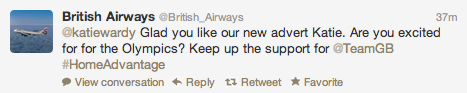
\includegraphics[width=1\textwidth]{mention_reply_example_figure}
  \caption[Example of a Twitter mention and @reply]{This tweet is an @reply to a user named `katiewardy' but also contains a mention of a user named `TeamGB', the official Twitter page for the United Kingdom's Olympic Team}
\label{fig:mention_reply}
\end{figure}
\end{center}



\paragraph{Retweets}

The final major feature of Twitter is yet another syntactic convention that was developed naturally by users and then given native support by Twitter: the retweet. A retweet is when a user repeats a tweet by another user to pass it along to their own followers, analogous to the re-sharing feature on Facebook. The common syntax is `RT @username [original tweet]', with the RT standing for retweet. The retweet is often sent along with a comment from the person retweeting about how they feel about what was said. While no specific convention exists for where to place this comment, two conventions often seen are to place a comment before the RT and to place it after the original tweet with some indication of the divide between the original tweet and the comment such as `//' or `...'. Figure~\ref{fig:retweet_hashtag} contains a screenshot of a tweet which includes a retweet which follows the convention of placing a comment before the RT.

\begin{center}
\begin{figure}
  \centering
  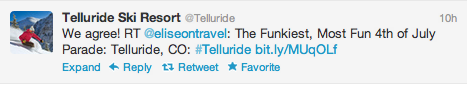
\includegraphics[width=1\textwidth]{retweet_hashtag_example_figure}
  \caption[Example of a Twitter retweet and hashtag]{An example of a Twitter retweet. Here, the resort has forwarded the positive tweet by user `eliseontravel' along with a comment of `We agree!' to their own followers. This tweet is also an example of a tweet containing a hashtag which was used in the original tweet: `\#Telluride'. The 'bit.ly/MUqOLf' at the end is a shortened link to an external website.}
\label{fig:retweet_hashtag}
\end{figure}
\end{center}


\subsubsection{Content Recommendation}

All of these features of the Twitter network are useful in content recommendation, and many of them have been used in existing studies as described in section~\ref{sec:ContentRecommendationResearch}. The primary advantage of the Twitter network as an object of study, however, is that the data is freely available and accompanied by an extensive API to allow the data to be queried and searched. This API has been used by numerous researchers to download large sets of tweets and the social graph accompanying it indicating which users follow which other users.

In fact, while studying Twitter it is actually a case of having far too much data to deal with easily than of not having enough data. Even though each tweet is no more than 140 characters, if the assumption is made that 100 million tweets are produced on a particular day (a very low estimate with today's usage), then that single day will contain roughly 14GB of data. Fortunately, previous researchers such as \cite{Kwak2010} and \cite{Choudhury2010} have already created some parsed versions of the data that can be used. More recently, a track of the Text Retrieval Conference (TREC)\footnote{http://trec.nist.gov/tracks.html} has been opened with regards to microblog research along with an enormous database of tweets from 2011. Though these datasets are all extremely large and thus useful for research, they still represent only a small fraction of the total data present.

This vast amount of readily available data meant that Twitter was by far the best option to study in this project, even though most of the concepts would be simple to apply to other social networks given the data since most of them have their major features in common with Twitter. As such, the remainder of this chapter will focus on Twitter since it is the object of study for this dissertation.


\section{Existing Research on Social Networks}

Twitter's simple and compact format and vast quantity of data has made it a popular target for research. The main topics of research are on the nature of the Twitter network itself, whether it is possible to gather useful information from Twitter, methods for determining what topics interest a particular Twitter user, and methods for ranking and recommending both tweets and users.

\subsection{The Twitter Network}

One of the earliest studies of the Twitter network was that of \cite{Java2007}, from 2007, only a few months after the service launched. The study was undertaken when Twitter had fewer than 100,000 users and during the two month study period only 1.3 million tweets were made. Clearly things have changed since this study, but it does still provide a number of interesting results. For example, they found that Twitter showed a high degree correlation---users with a large number of followers also tended to have a large number of followees. In the same vein, the distribution of indegree and outdegree had a similar power exponent to that of the web and the blogosphere.

The most important findings of \cite{Java2007} were the different categories of users and of content. They found that the content produced mostly fell into four different categories: daily chatter, conversations, sharing information, and reporting news. Importantly, conversation comprised nearly one-eighth of the tweets in their dataset. Presumably if a similar study were repeated today it would find a fifth content category: spam. Users were found to fall into three categories: information seekers, users who may tweet infrequently but still commonly check the site for the tweets of others; information sources, users who post information that others find valuable; and friends. At the time of the study friendship links constituted most of the links between users, though with more than 100 million users today, this is unlikely to be the case.

A later study by \cite{Cha2010} indirectly speaks to how much growth Twitter underwent between 2007 and 2010. At the time of that study in August 2009 Twitter had grown to nearly 54 million active users with 1.9 billion links between them and more than 1.7 billion tweets. The threshold for popularity investigated here, one million followers, is more than ten times greater than the total number of users in the 2007 study of \cite{Java2007}. \cite{Cha2010} found that while Twitter users with one million followers might seem intuitively to be the most influential, the number of followers alone was in general a poor measure of the influence that a user has.

\cite{Welch2011}, a 2011 study, investigated which links in the twitter network (e.g. follower links, retweet links, etc.) were most likely to preserve topical relevance. They found that the most important link type for preserving this topical relevance is retweet links. Crucially, they also found that ``traversing even a single follow link dramatically reduces the probability of topical relevance". In carrying out this study they repeated some of the experiments of \cite{Java2007} and found that most of the results from there still held true, despite the massive growth of the service.

A very important study for the purposes of this project is that of \cite{Kwak2010}, an in-depth examination of characteristics of the Twitter network. In many ways it is similar to the early 2007 study of \cite{Java2007}, but with a much more mature network. They studied things such as how likely a user was to reciprocate when someone followed them, the relationship between followee/follower numbers and number of tweets, the distribution of followee/follower numbers, the nature of trending topics, and the reasons behind and impacts of retweets, among other topics.

An important result from this study is that the number of followers/followees that users have behaves according to a strong power law with a long tail. There are hundreds of thousands of users with fewer than ten or twenty followers or followees, while only 40 users at the time of the study had more than one million followers. And of the users, 67\% were not followed by any of their followees! The results also showed that how many tweets a user had was a strong predictor of both how many followers and how many followees that person had, at least up to about 100 follower or followees.

Those results are interesting, but the crucial outcome of \cite{Kwak2010} for this project is the large dataset that was produced in order to find those results, of which the complete social graph (more than 1.2 billion edges) which was included and used for this project is the most important component. The social graph from this study was the main one used in the project, as discussed in Section~\ref{sec:SelectingADataset}.


\subsection{Gathering Information From Twitter}
\label{sec:InfoGatheringResearch}

Given the vast size of the Twitter network and the vast amount of data produced by its users in talking about what they are doing and how they feel, it is not surprising that studies have been undertaken to try to mine this data to gain more insight into what people believe and what they're discussing.

The study undertaken by \cite{O'Connor2010} attempted to predict the results of opinion polls based only on Twitter data. This process makes perfect sense when one considers that an opinion poll is really just an attempt to determine how a large population feels about something by sampling a small portion of that population and asking them how they feel. Analysing Twitter data, then, is akin to asking a much larger sample of that population.

Using a dataset of one billion tweets collected in 2008 and 2009, the research investigated three different possible opinion applications: election polls, job approval polls, and consumer confidence. For each application, tweets were analysed from a relevant period of time, such as in the run-up to the presidential election. For each tweet that contained certain trigger words that indicated relevance to a particular poll, the sentiment was analysed by simply seeing if a tweet had positive or negative words. All of the scores both positive and negative for a given period were summed and amalgamated and then compared to opinion polls from the same period of time.

The results were not perfect but did show a strong correlation for both job approval ratings and consumer confidence. Predicting election polling proved to be a more difficult task, and the correlation on those polls was not nearly as good. The strength of these results based on a very rudimentary method of sentiment analysis suggests that better techniques for analysing the tweets could improve the results.

A similar study was performed in \cite{Asur2010}, this time to try to predict the box office gross revenue of films. This study also reported some promising results from mining the sentiment of vast numbers of tweets in order to determine peoples' opinions.


\subsection{Determining User Interest}
\label{sec:UserInterestResearch}

A number of studies have focused on determining which topics are most often discussed by a user and which topics a user is most interested in reading about. The techniques from this area are very useful to the work undertaken in this project, particularly in determining the similarity of different pieces of content, e.g. as used in Section~\ref{sec:ProjectingToBipartite}. Section~\ref{sec:DeterminingContentSimilarity} describes the use of named-entity recognition (NER) for purposes of determining which tweets are related, but any of the techniques used in this section could be used instead, probably with better results, albeit at the expense of greater run times.

One study, \cite{Michelson2010}, used an ontology-based approach to determine a user's topics of interest. In this case, the ontology was the category structure of Wikipedia. For each tweet by a particular user, named entities were found using a named-entity recognizer. Those entities were then looked up in Wikipedia in order to disambiguate them and determine their categories. After repeating this process for all tweets by a user the process yields a pretty good set of the top ten topics of interest to that user.

A more mathematical approach was taken by \cite{Ramage2010}. They used a partially supervised machine learning algorithm and achieved good results when categorizing the tweets. Their particular machine learning approach was Labelled Latent Dirichlet Allocation, which finds distributions of words which tend to occur in similar documents. These sets of similar words are taken to be the topics, and the topics of interest to particular users can determined by analysing their tweets for these words. The authors were unsure at the outset if this technique, commonly used for long documents such as news articles, would work for documents as short as tweets, and their results indicate that it is quite successful.

A more recent method, \cite{Pochampally2011}, attempted to determine the topics of interest for a particular distinguished user by finding which of their followees were most important and setting the topics discussed by those users as the topics of interest for the distinguished user. The study used an approach based primarily on the Twitter network, including follower/followee relationships and retweet/mention relationships in order to determine the list of top users. As in other studies, retweets were found to be the most reliable and were thus weighted the most heavily. Upon identifying the top users, they took an approach similar to that of \cite{Michelson2010}, using Wikipedia to look up terms and disambiguate them, though they used nouns returned from a part-of-speech tagger rather than named-entity recognition.


\subsection{Content and User Recommendation}
\label{sec:ContentRecommendationResearch}

Two main approaches exist in current research on recommending content and users, the network-based approach and the content-based approach. In the network-based approach, the connections between users and their interactions with one another via retweets and mentions form the primary basis for recommendation. In the content-based approach, meanwhile, the analysis is primarily focused on the tweets themselves, such as by determining which tweets are most similar to one another. The two approaches are by no means mutually exclusive and are often used in complementary ways.

The research described here shows that when recommending users and content, each approach has had some degree of success.

\subsubsection{Recommending Users}

\cite{Kwak2010}, the wide-ranging study that provided the dataset used for this project, included some analysis of potential network-based techniques for ranking users, though it was not the primary focus of the study. They used several techniques: ranking users in terms of number of followers, running the PageRank algorithm on the social graph, and ranking users in terms of how many times their content had been retweeted. As expected based on the results of \cite{Welch2011}, the number of retweets was the best of these ranking schemes. PageRank and the number of followers metric produced nearly identical results, suggesting based on the results of \cite{Cha2010}---namely that a user's number of followers is a poor measure of their influence---that PageRank is not a good technique to use for recommending users.

Still, PageRank has been used by other studies, such as in \cite{Weng2010}. They called their method TwitterRank because it differed slightly from original PageRank. Rather than visiting all users with uniform probability over links as in the random walk of PageRank, TwitterRank performs a topic-specific random walk using topics derived using Latent Dirichlet Allocation. Their results indicate that this modification allowed TwitterRank to outperform both the PageRank metric and a metric based on the indegree of nodes when ranking tweets. The performance improvement over page rank was small, however.

A hybrid approach utilizing both network and content information was taken by \cite{Armentano2011}. The goal of the research was to provide user recommendations in some sort of a ranked order. A network based approach was taken first in order to  discover potentially interesting users. From that unordered list of potentially interesting users a ranked list is created by comparing the users based on the content that they produce to a reference document of what the user is interested in. Two strategies specifically used for building the user profile are the user's own tweets and the tweets of the user's followees.

Another piece of work focused on recommending users is presented in, \cite{Hannon2010}, which recommends users based purely on content. As with a number of other approaches, the major choice explored is what to use as the reference content to which other users are compared. Several different strategies are compared, some of them overlapping with those examined by \cite{Armentano2011}. The tweets of the user, their followees, and their followers were all considered, as were the lists of users' followers and followees. Additionally, combinations of these methods were employed in a hybridized approach. For each means of building them, the user profile documents were compared as TF-IDF valued word vectors (see Section~\ref{sec:ContentScoringMethod} for more details on TF-IDF weighting). The hybrid approaches performed the best, generally speaking. 

\subsubsection{Recommending Content}

Attempts to rank individual tweets have also been made, such as in \cite{Duan2010}, which used a content-based approach to this recommendation. Here, various content features are gathered for each tweet and then a learning algorithm is employed to evaluate which of these features should be ranked most highly. The various features that were evaluated can be divided into three basic groups: those based on the content of the tweets themselves, those based on Twitter-specific features, and those based on the authority of the users who created the tweet.

The features for the content of the tweets were represented by the Okapi BM25 or cosine similarity score between a tweet and a query being evaluated. The twitter-specific group included features such as the length of the tweet, whether it contained hashtags, whether it contained a URL, and how many times it had been retweeted. Finally, the account authority group included metrics such as how many followers the author of the tweet has and their PageRank score within the twitter network. Surprisingly, the mere presence of a URL was found to be the most important feature, and the length of the tweet was also found to be very predictive.

\subsubsection{Recommending Both Users And Content}

The work of \cite{Kim2011} used a machine learning algorithm to recommend both users and specific content in a system that they called TWITOBI. The approach is primarily based on the content of tweets, but some information about who follows whom in the network is utilized. A probabilistic model based on the expectation maximization algorithm is trained to properly rank both tweets and users via a similar technique. 

The sample size in terms of number of users was fairly small, consisting of only 8,405 users, but the sample size in terms of number of tweets was very large, with more than 12 million tweets by those 8,405 users. No discussion of how those users were decided upon is included, which when combined with the small number of users makes some of the results a bit suspect.

\subsubsection{Common Threads}

Many of the methods for recommending users and content utilize similar ideas in making their recommendations. The literature indicates via multiple studies that retweets are a very important predictor of what a user is interested in and that retweets are also an excellent indicator of how much influence a user has over others. It is also clear from existing research that the PageRank algorithm, while useful to some degree, does not perform very well at predicting which users will be most influential on a given user.

Most recent research has not focused specifically on either the network-based approach or the content-based approach, preferring instead to take useful features from each. This dissertation takes the same tack, utilizing useful features from both the network and the content. In many cases, features used successfully in the research reviewed here were not used for various reasons, but would make excellent additions to the methodology and implementation described in chapters 3 and 4.




